\section*{Problem \#4}


Consider the nonlinear system:
$$
\dot{x}=f(x), \quad x(0)=x_{0}
$$
where $f(0)=0 .$ Assuming that $f: D \rightarrow \mathbb{R}^{n}$ is Lipschitz on its domain and let solutions of the system be bounded by:
$$
\|x(t)\| \leq \beta(\|x(0)\|, t)
$$
for $\|x(0)\|<c$ for some $c>0$ where $\beta \in \mathcal{K} \mathcal{L} .$ Show that the origin is asymptotically stable in the sense of the classical asymptotic stability $(\epsilon-\delta)$ definition.



\begin{center}
  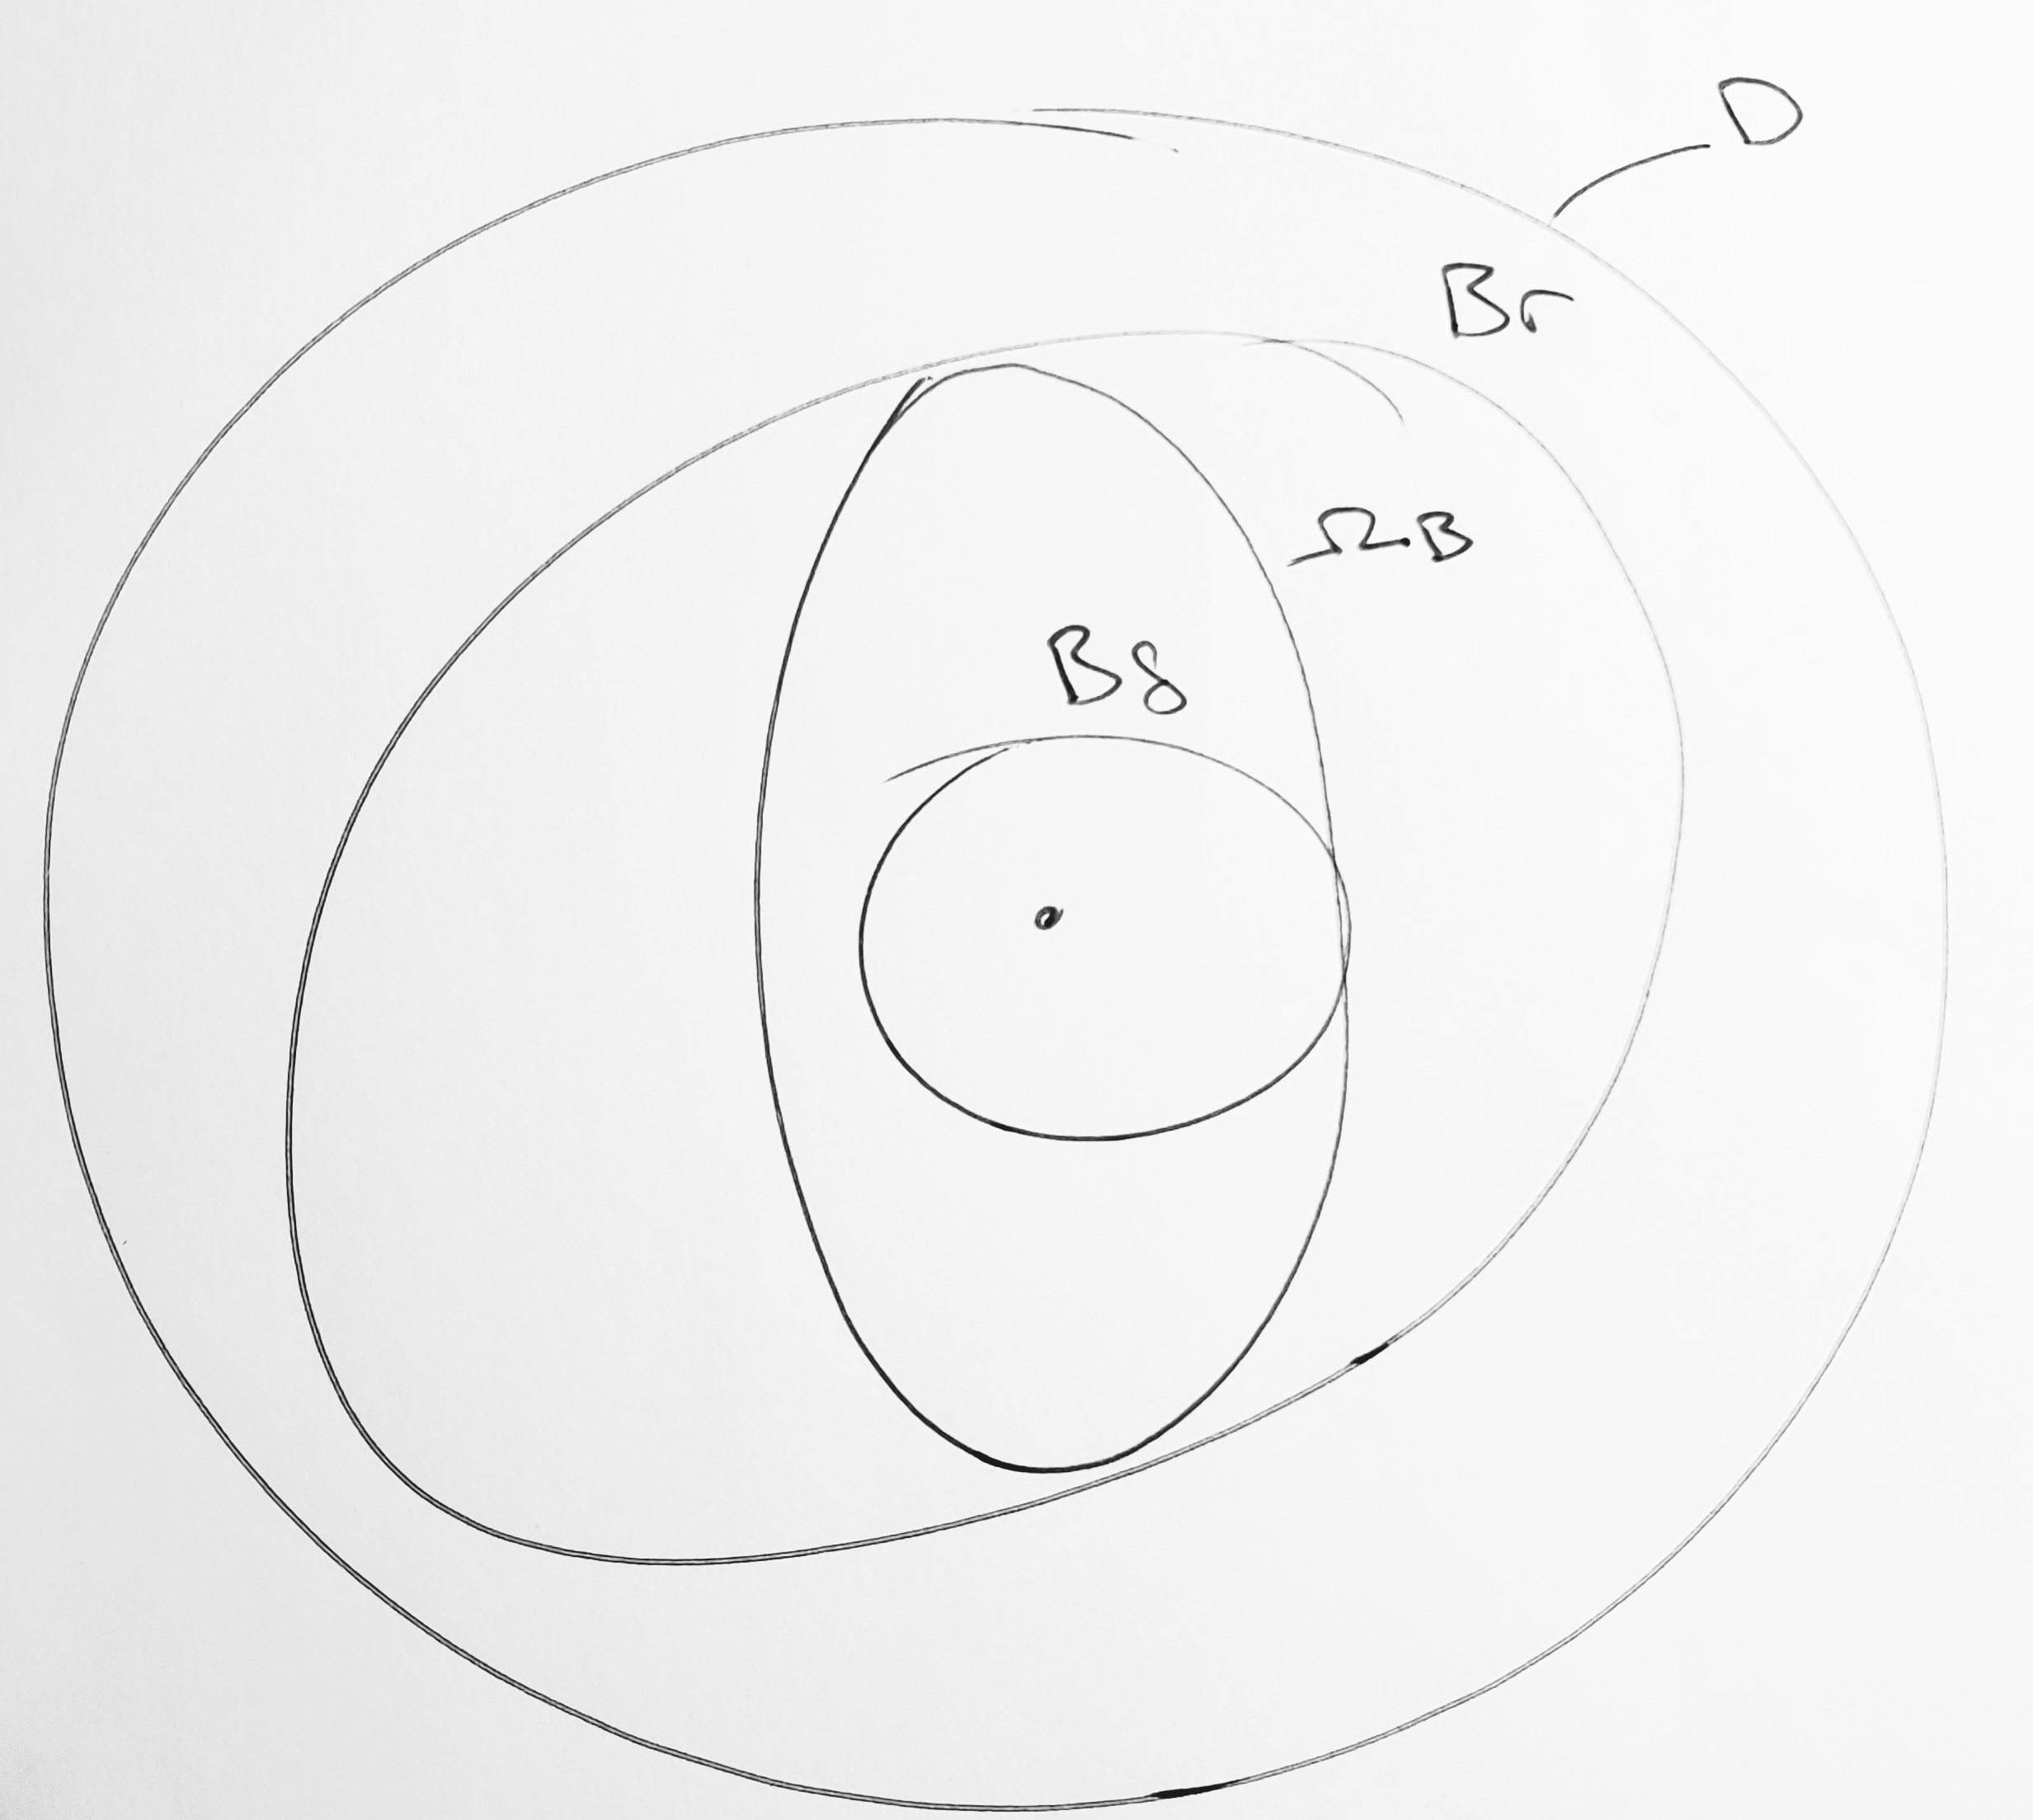
\includegraphics[scale=0.1]{proof}
\end{center}

\noindent In order to demonstrate that the system (as defined using Comparison functions) is asymptotically stable, we need to demonstrate the $\epsilon - \delta$ proof of asymptotic stability and relate that to the usage of comparison functions to show the equivalence between the two. \\

\noindent For $\epsilon >0$ such that $r \in (0, \epsilon]$

$$
B_r = \{ x\in \R^n | \left\Vert x \right\Vert < r\} \subset D
$$

\noindent Then there is an $\alpha = min_{\left\Vert x \right\Vert = r} V(x)$, non-negative $\alpha >0$, such that $\beta \in (0, \alpha)$ we can define a positive invariant set $\Omega_B$ such that


$$
\Omega_B = \{ x \in B_r | V(x) \leq \beta\}
$$

\noindent Note that since, $\Omega_B$ is an invariant set, it has the property that any trajectory starting in it $x(t_0)$ remains in it such that $\left\Vert x(t) \right\Vert \in \Omega_B$. Due to this property we know that there must exist a function which is strictly decreasing such that ...


$$
V(x(t)) \leq V(x(t_0)) \leq \beta \quad \quad \forall t \leq t_0
$$

\noindent In order for this to be true

$$
\dot{V}(x) \leq 0
$$

\noindent It should be noted that $\Omega_B$ is a compact set by construction since it is a subset of $B_r$. From this fact, and under the assumptions listed in the problem statement, we can say that $\dot{x} = f(x)$ has a unique solution $\forall t \geq t_0$ for $X(t_0) \in \Omega_B$.\\

\noindent If $V(x)$ is continuous and $V(0) = 0$, we can define a $\delta$ such that..

$$
\left\Vert x \right\Vert \leq \delta \Rightarrow V(x) < \beta
$$

\noindent Since we know that ball of radius $\delta$ infers a value of $V(x)$ inside of ball of radius $\beta$, we can show that...

$$
B_{\delta} \subset \Omega_B \subset B_r
$$

\noindent If we start a trajectory inside of the ball of radius $\delta$ we can show that

$$
x(t_0) \in B_{\delta} \Rightarrow x(t_0) \in \Omega_B \Rightarrow x(t) \in \Omega_B \Rightarrow x(t) \in B_r
$$

\noindent This means that given this setup, from a given $\delta$ there must exist a $\epsilon$ (recall: $B_r$ defines the $\epsilon$) such that we can state.

$$
\left\Vert x(t_0) \right\Vert < \delta \Rightarrow \left\Vert x(t) \right\Vert < r \leq \epsilon, \quad \quad \forall t \geq t_0
$$


\noindent If this is true such this means that the system is stable according to the $\epsilon-\delta$ definition. However, this does not show that system is \underline{attractive}. In order to show that we need to prove that...

$$
x(t) \rightarrow 0 \quad \text{ as } t \rightarrow \infty
$$


\noindent Since the function $V(x(t))$ is decreasing we can show that if ...

$$
V(x(t)) \rightarrow c \geq 0 \text{ as } t \rightarrow \infty
$$

\noindent It is sufficient to show that the function $V(x) \rightarrow 0 $ as $t \rightarrow \infty$.

\subsection*{Solution Problem 4}

With the structure of the main proof out of the way, we need to show how the \underline{comparison functions} can be linked to this definition for asymptotic stabiilty. We can show that we can define the functions $V(t,x)$ and $\dot{V}(t,x)$ in terms of the comparison function $\alpha_i \in K$ and $\beta_i \in KL$. From the definitions of the classes (K, KL) we can show that in order for the function $V$ to be positive definite it must be able to be upper and lower bounded by functions $\alpha_1(\cdot)$ and $\alpha_2(\cdot)$. \\

$$
\alpha_1(\left\Vert x \right\Vert) \leq V(t,x) \alpha_2(\left\Vert x \right\Vert)
$$

\noindent In addition to this, we must show that the function $\dot{V}(x)$ is negative definite, which can be stated as $\dot{V} \leq -\alpha_3(\cdot)$. We can observe that via Lemma 4.2, that by using properties of these functions we can rewrite

$$
V(t,x) \leq \sigma(V(t_0, x(t_0)), t- t_0), \quad \forall V(t_0, x(t_0)) \in [0,c]
$$

\noindent which can be written

$$
\left\Vert x \right\Vert \leq \beta(\left\Vert x(0)\right\Vert, t)
$$

Since it is possible to rewrite the original statement of asymptotic stability in terms of comparison functions, we can show the direct connection between the form of the problem given and the direct $\epsilon-\delta$ proof of asymptotic stability.
